% !TEX program = lualatex
% ============================================================
% UNIVERSAL MAINFRAME — σₚ Framework
% Author: Adrian Zander (2025)
% ============================================================

\documentclass[11pt,a4paper]{article}

% --- Page layout & language ---
\usepackage[a4paper,margin=2.3cm]{geometry}
\usepackage[english]{babel}
\usepackage{fontspec}
\setmainfont{TeX Gyre Termes}
\usepackage{microtype}
\usepackage{csquotes}

% --- Mathematics ---
\usepackage{amsmath,amssymb,amsthm,mathtools}
\usepackage{physics}
\usepackage{siunitx}
\sisetup{locale=US,detect-all}

% --- Graphics & Plots ---
\usepackage{graphicx}
\usepackage{xcolor}
\usepackage{tikz}
\usetikzlibrary{arrows.meta,calc,decorations.pathmorphing,positioning}
\usepackage{pgfplots}
\pgfplotsset{compat=1.18}
\usepackage{bm}
\usepackage{booktabs}
\usepackage[most]{tcolorbox}

\usepackage{tocloft}
\usepackage{hyperref}
\usepackage{bookmark}

% ToC style
\renewcommand{\cfttoctitlefont}{\Large\bfseries}
\renewcommand{\cftsecfont}{\bfseries}
\renewcommand{\cftsubsecfont}{\itshape}
\setlength{\cftbeforesecskip}{4pt}

% Hyperlinks
\hypersetup{
  colorlinks=true,
  linkcolor=blue!50!black,
  urlcolor=cyan!60!black,
  citecolor=black,
  pdfauthor={Adrian Zander},
  pdftitle={A Requiem for LCDM – σₚ Framework},
  pdfsubject={Unified Quantum–Relativistic Model},
  pdfkeywords={sigma_P, quantum gravity, cosmology, Planck scale, Zander equation}
}

\setcounter{tocdepth}{2}
\setcounter{secnumdepth}{2}

% --- Macros: constants & σₚ structure ---
\newcommand{\lp}{\ell_{\mathrm{P}}}
\newcommand{\tp}{t_{\mathrm{P}}}
\newcommand{\mpP}{M_{\mathrm{P}}}
\newcommand{\sigmaP}{\sigma_{\mathrm{P}}}
\newcommand{\alphaSigma}{\alpha_{\sigma}}
\newcommand{\Lambdaeff}{\Lambda_{\mathrm{eff}}}
\newcommand{\GNewton}{G}
\newcommand{\kb}{k_{\mathrm{B}}}
\newcommand{\TZ}{\Theta_{\mathrm{Z}}}

% Metric signature: (-,+,+,+)
\newcommand{\signatur}{(-,+,+,+)}

% --- Theorems ---
\theoremstyle{definition}
\newtheorem{definition}{Definition}
\theoremstyle{remark}
\newtheorem{remark}{Remark}
\theoremstyle{plain}
\newtheorem{theorem}{Theorem}

% --- Bibliography ---
\usepackage[backend=biber,style=phys,biblabel=brackets]{biblatex}
\addbibresource{references.bib}

% ============================================================
% Title
% ============================================================
\title{
  \vspace{-1em}
  \Large A Requiem for ΛCDM\\[0.5em]
}
\author{Adrian Zander}
\date{October 2025}

\begin{document}
\maketitle

\section*{Status / Einordnung}
\noindent\textbf{Document type:} Conceptual Essay / Position Paper (working draft)\\
\textbf{Claim level:} Interpretive and hypothesis driven. Scientific and cosmological claims require separate derivations, uncertainty estimates, and independent data-model comparison.\\
\textbf{Use:} Use for conceptual framing and hypothesis generation, not as a final empirical claim document.


% ============================================================
% Abstract
% ============================================================
\begin{abstract}
For almost a century, we have described the universe in separate languages:
quantum mechanics for the small, general relativity for the large,
and cosmological parameters as fudge factors in between.
The standard cosmological model, $\Lambda$CDM (Lambda Cold Dark Matter), has been an extraordinarily successful
effective description. Yet precise measurements (Planck, SH0ES, weak lensing,
SPARC, LIGO) and the first deep fields of the James Webb Space Telescope\cite{JWST2023Mission} suggest:
we observe a universe that is too early, too structured, too coherent, and too stable
to be merely the outcome of a finely tuned vacuum term and invisible components.
\newline
This work develops a consistent alternative that requires neither additional fields
nor free parameters. The starting point is not a hypothetical new particle,
but the finite structure of spacetime itself. The fundamental cell
\[
  \sigmaP = \lp\,\tp = \frac{\hbar \GNewton}{c^4}
\]
is interpreted as the natural quantum of spacetime action.
From this follows a dimensionless spacetime fine-structure constant
\[
  \alphaSigma = \frac{\sigmaP}{R t} \approx 10^{-123},
\]
and a geometric cosmological constant
\[
  \Lambdaeff = \frac{3}{c R t},
\]
arising directly from the finiteness of the observable universe.
The so-called “vacuum catastrophe” disappears: local quantum fluctuations and
macroscopic curvature emerge as two consistent scales of the same geometry.
\newline
On this basis, a fully quantized field equation is formulated,
where gravitation, quantum fields, and thermodynamic information are linked
through a single invariant measure — $\sigmaP$.
A central element is the Zander functional temperature
\[
  \TZ(M) = \frac{c^3}{8\pi \GNewton\, M\, \kb\, \hbar},
\]
which describes not a divergent energy flux, but the continuous exchange of
spacetime action per unit mass.
It rises during the evaporation of a black hole up to the Planck mass,
then decreases again, leaving a stable remnant that stores information.
The resulting dynamics yield:
a smooth Page curve (unitary information flow),
finite curvature at all scales (no singularities),
and a natural explanation for $\Lambdaeff = 3/(c R t)$.
\newline
Within this framework, black holes do not appear as the endpoints of physics,
but as organized memory structures of spacetime.
The universe does not forget:
\newline
It radiates, stores, and evolves in geometric harmony.
\newline
All results are derived solely from the natural constants 
$\{\hbar,\, c,\, G,\, k_{\mathrm B}\}$, from their natural units, and from
empirically verifiable observations.
\end{abstract}

% ============================================================
% Legend of Symbols and Signature Equations
% ============================================================
\clearpage
\section*{Legend of Symbols and Signature Equations}
\addcontentsline{toc}{section}{Legend of Symbols and Signature Equations }

% --- Box 1 ---
\begin{tcolorbox}[
  colback=white,
  colframe=black!70,
  arc=2mm,
  boxrule=0.5pt,
  title={\bfseries Fundamental Constants and Planck Units\cite{Planck1901}}]

\begin{align*}
c &\approx 2.998\times10^8~\mathrm{m/s}
&\text{speed of light}\\[2pt]
G &\approx 6.674\times10^{-11}~\mathrm{m^3/(kg\,s^2)}
&\text{gravitational constant}\\[2pt]
\hbar &\approx 1.055\times10^{-34}~\mathrm{J\,s}
&\text{reduced Planck constant}\\[2pt]
k_{\mathrm B} &\approx 1.381\times10^{-23}~\mathrm{J/K}
&\text{Boltzmann constant}
\end{align*}

\begin{align*}
\ell_{\mathrm P}
&= \sqrt{\frac{\hbar G}{c^3}}
&\text{Planck length}\\[2pt]
t_{\mathrm P}
&= \sqrt{\frac{\hbar G}{c^5}}
&\text{Planck time}\\[2pt]
M_{\mathrm P}
&= \sqrt{\frac{\hbar c}{G}}
&\text{Planck mass}\\[2pt]
\sigma_{\mathrm P}
&= \ell_{\mathrm P}t_{\mathrm P}
= \frac{\hbar G}{c^4}
&\text{spacetime quantum}
\end{align*}
\end{tcolorbox}

\vspace{0.8em}

% --- Box 2 ---
\begin{tcolorbox}[
  colback=white,
  colframe=black!70,
  arc=2mm,
  boxrule=0.5pt,
  title={\bfseries Geometry: Minkowski–Zander and Field Equations\cite{Zander2025_ProblemOfTime}}]

\paragraph{Minkowski spacetime.}
\begin{align*}
ds^2 &= c^2 dt^2 - dx^2 - dy^2 - dz^2,\\
\gamma(v) &= \frac{1}{\sqrt{1-v^2/c^2}}.
\end{align*}

\paragraph{Spacetime uncertainty.}
\[
\Delta x\,\Delta t \ge \sigma_{\mathrm P}.
\]

\paragraph{Minkowski–Zander metric.}
\begin{align*}
\tilde{g}_{\mu\nu}(x)
&= \frac{g_{\mu\nu}(x)}{1+\sigma_{\mathrm P}^{-1}f(\mathcal{R}(x))},\\
d\tilde{s}^2 &= \tilde{g}_{\mu\nu}dx^\mu dx^\nu.
\end{align*}

\paragraph{Einstein–Zander equation.}
\begin{align*}
\left\langle
\widehat{G}_{\mu\nu}
+ \Lambda_{\mathrm{eff}}(W)\,g_{\mu\nu}
\right\rangle_{\sigma_{\mathrm P}}
&=
\frac{8\pi G}{c^4}
\left\langle
\widehat{T}_{\mu\nu}
\right\rangle_{\sigma_{\mathrm P}}^{(W)},\\
\Lambda_{\mathrm{eff}}(W)
&= \frac{3}{c R t}.
\end{align*}

\paragraph{Classical limit.}
\[
G_{\mu\nu} + \Lambda_{\mathrm{eff}}g_{\mu\nu}
= \frac{8\pi G}{c^4}\bar T_{\mu\nu}.
\]
\end{tcolorbox}

\vspace{0.8em}

% --- Box 3 ---
\begin{tcolorbox}[
  colback=white,
  colframe=black!70,
  arc=2mm,
  boxrule=0.5pt,
  title={\bfseries Black Holes, Entropy and Zander Functional}]

\paragraph{Schwarzschild radius.}
\[
r_s = \frac{2GM}{c^2}.
\]

\paragraph{Bekenstein–Hawking entropy.}
\[
S_{\mathrm{BH}} = \frac{k_{\mathrm B}A}{4\ell_{\mathrm P}^2},
\quad A = 4\pi r_s^2.
\]

\paragraph{Hawking temperature.}
\[
T_H(M) = \frac{\hbar c^3}{8\pi G M k_{\mathrm B}}.
\]

\paragraph{Zander functional.}
\[
\Theta_Z(M) = \frac{c^3}{8\pi G M k_{\mathrm B}\hbar}.
\]
Finite spacetime action flow per mass unit:
instead of a divergent temperature, a stable remnant forms at $M\!\sim\!M_{\mathrm P}$.\cite{Zander2025_MemoryOfSpacetime}

\end{tcolorbox}

\vspace{0.8em}

% --- Box 4 ---
\begin{tcolorbox}[
  colback=white,
  colframe=black!70,
  arc=2mm,
  boxrule=0.5pt,
  title={\bfseries Cosmological Scaling from $\sigma_{\mathrm P}$}]

\paragraph{Planck-cell curvature.}
\[
\Lambda_{\mathrm{cell}} = \frac{3}{\ell_{\mathrm P}^2}.
\]

\paragraph{Number of spacetime cells.}
\[
N_\sigma = \frac{R\,t}{\sigma_{\mathrm P}} = \frac{R\,t\,c^4}{\hbar G}.
\]

\paragraph{Macroscopic cosmological constant.}
\[
\Lambda_{\mathrm{geo}} = \frac{\Lambda_{\mathrm{cell}}}{N_\sigma}
= \frac{3}{c R t}.
\]
The apparent “vacuum catastrophe” vanishes:
local QFT vacuum energy and observed $\Lambda$ are two scales
of the same σ$_{\mathrm P}$ geometry.\cite{Zander2025_ParameterFreeUnification}
\end{tcolorbox}

\begin{figure}[ht]
    \centering
    \includegraphics[width=0.4\linewidth]{Universe.jpg}
    \caption{
        \textbf{Spherical representation of a quantized universe.}
           }
\end{figure}

\clearpage
\section{Introduction}

At the end of the 20th century, cosmology believed it had made peace with the universe.  
Saul Perlmutter, Adam Riess, and Brian Schmidt\cite{Perlmutter1999,Riess1998}
observed that distant supernovae appeared dimmer than expected from a purely gravitationally decelerating expansion.  
The interpretation: the universe is accelerating.  
This apparent anomaly was not taken as a sign of an incomplete theory, but as an opportunity to postulate a missing form of energy — \emph{dark energy}.
\newline
Thus began one of the strangest episodes in the history of science:  
theoretical physics celebrated the discovery of an “accelerating cosmos” without knowing its cause, and the standard model of cosmology — the so-called $\Lambda$CDM model — elevated darkness to a principle.  
$\Lambda$ (Lambda) henceforth stood for a cosmological constant whose observed value was 123 orders of magnitude smaller than the theoretical vacuum energy predicted by quantum field theory.  
The \emph{greatest discrepancy in physics} was promptly declared an empirical virtue.
\newline
Yet while the theories congratulated themselves, the universe began to look back.  
With the \emph{James Webb Space Telescope} (JWST), humanity gained a view into the first 300~million years after the Big Bang — and found something that should not have existed:  
fully developed galaxies with high metallicity, rotating disks, and complex structures that, according to all LCDM simulations, should have taken billions of years to form.  
The telescope that was meant to confirm dark-energy cosmology is now shaking the most elegant fiction of modern astrophysics.
\newline
Darkness, it turns out, was never a property of the universe — it was a symptom of our equations.  
It was not the cosmos that was incomplete, but our mathematical grid, in which space and time were still treated as infinite, continuous quantities.  
The solution lies not in an additional field, but in the structure of spacetime itself.
\newline
This work demonstrates that a single, yet fundamental relation connects all essential phenomena:
\[
\sigma_{\mathrm P} = \ell_{\mathrm P}t_{\mathrm P} = \frac{\hbar G}{c^4}.
\]
This quantum of spacetime action — the smallest possible product of space and time — defines the natural limit of physical divisibility.  
From this finite structure follows a geometric, parameter-free explanation of cosmic acceleration:
\[
\Lambda_{\mathrm{geo}} = \frac{3}{c R t}.
\]
It describes not an unknown energy field, but the intrinsic measure of finite spacetime itself.
\newline
Where $\Lambda$CDM derives its darkness from missing data and hypothetical particles,  
the $\sigma_{\mathrm P}$ framework derives the same acceleration from quantized geometry — from the fact that spacetime cannot be divided arbitrarily.  
As a result, the vacuum problem disappears, the Hubble tension is naturally embedded,  
and the JWST observations\cite{JWST2023EarlyGalaxies} no longer appear as anomalies,  
but as direct confirmations of a finite, self-consistent spacetime.
\newline
The universe is not dark.  
\newline  
It is quantized.

\subsection*{On the Purity of the Equation}

Einstein’s field equation\cite{Einstein1915} was never merely a computational rule.
It is a statement about nature’s balance:
\[
G_{\mu\nu} + \Lambda g_{\mu\nu}
= \frac{8\pi G}{c^4}\,T_{\mu\nu}.
\]
On the left stands geometry — space itself, as it curves;
on the right, matter — that which shapes it.
Einstein’s genius did not lie in the symbol $\Lambda$,
but in the symmetry of this equilibrium.
\newline
In the late 20th century, this balance was broken.
To explain the presumed accelerated expansion,
$\Lambda$ was moved to the matter side
and reinterpreted as \emph{dark energy}.
The equation remained correct,
but its meaning was desecrated:
a geometric principle was redefined as a fluid.
\newline
Within the $\sigma_{\mathrm P}$ framework, this bookkeeping error is corrected.
$\Lambda$ is not a form of energy,
but the signature of a finite spacetime:
\[
\Lambda_{\mathrm{geo}} = \frac{3}{c R t}.
\]
Dark energy disappears — 
not because it was measured incorrectly,
but because it was never on the right side of the equation
and therefore never existed.
\newline
Spacetime itself is the source of acceleration:
it does not expand because something drives it,
but because it acts anew at every moment.
The universe follows no pressure,
but the measure of its own geometry:
\[
\sigma_{\mathrm P} = \frac{\hbar G}{c^4}.
\]
Thus, the equation regains its purity.
Geometry and matter become once again two sides of the same reality —  
not separate, but quantized and connected.

\begin{quote}
\textit{One must never alter the geometric side of the equation —  
\newline 
for it is not a model, it is a law.}  
\\[0.5em]
And our later Nobel laureates should have known this.
\end{quote}

\vspace{1em}
\begin{center}
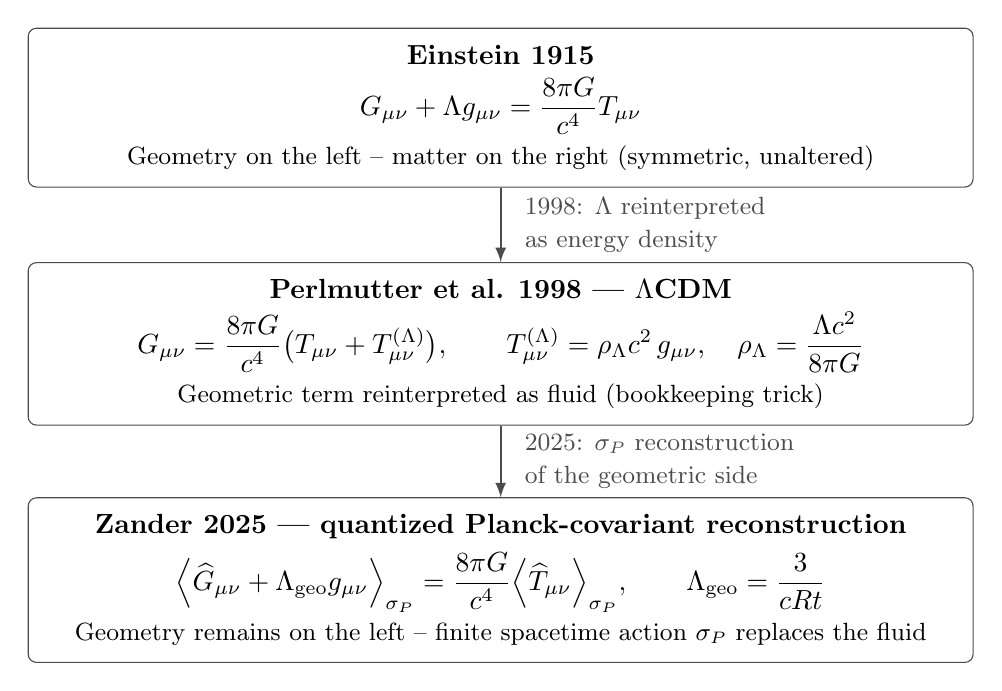
\begin{tikzpicture}[>=latex,scale=1.0]
\tikzstyle{eqbox}=[rectangle,rounded corners=3pt,draw=black!70,fill=white,
                   minimum width=12cm,minimum height=1.8cm,align=center,inner sep=6pt]
\tikzstyle{arrow}=[->,thick,black!70]

% --- Einstein 1915 ---
\node[eqbox] (einstein) at (0,5.5) {
\textbf{Einstein 1915}\\[0.4em]
$\displaystyle
G_{\mu\nu} + \Lambda g_{\mu\nu}
= \frac{8\pi G}{c^4} T_{\mu\nu}$\\[0.3em]
{\small Geometry on the left – matter on the right (symmetric, unaltered)}
};

% --- Perlmutter 1998 (ΛCDM) ---
\node[eqbox] (lcdm) at (0,2.5) {
\textbf{Perlmutter et al. 1998 — $\Lambda$CDM}\\[0.4em]
$\displaystyle
G_{\mu\nu}
= \frac{8\pi G}{c^4}
\big(T_{\mu\nu} + T^{(\Lambda)}_{\mu\nu}\big),
\qquad
T^{(\Lambda)}_{\mu\nu}
= \rho_\Lambda c^2\, g_{\mu\nu},
\quad
\rho_\Lambda = \frac{\Lambda c^2}{8\pi G}$\\[0.3em]
{\small Geometric term reinterpreted as fluid (bookkeeping trick)}
};

% --- Zander 2025 ---
\node[eqbox] (zander) at (0,-0.5) {
\textbf{Zander 2025 — quantized Planck-covariant reconstruction}\\[0.4em]
$\displaystyle
\Big\langle \widehat{G}_{\mu\nu}
+ \Lambda_{\mathrm{geo}} g_{\mu\nu} \Big\rangle_{\sigma_P}
= \frac{8\pi G}{c^4}
\Big\langle \widehat{T}_{\mu\nu} \Big\rangle_{\sigma_P},
\qquad
\Lambda_{\mathrm{geo}} = \frac{3}{c R t}$\\[0.3em]
{\small Geometry remains on the left – finite spacetime action $\sigma_P$ replaces the fluid}
};

% --- Arrows ---
\draw[arrow] (einstein.south) -- node[right,align=left,xshift=5pt]
  {\small 1998: $\Lambda$ reinterpreted \\ \small as energy density} (lcdm.north);
\draw[arrow] (lcdm.south) -- node[right,align=left,xshift=5pt]
  {\small 2025: $\sigma_P$ reconstruction \\ \small of the geometric side} (zander.north);

\end{tikzpicture}
\end{center}

\subsection*{Note on the Current Observational Status}

Since the “groundbreaking” measurements of \textcite{Perlmutter1999,Riess1998}, the accelerated expansion of the universe has been considered experimentally confirmed.  
In recent years, however, doubts about the robustness of this conclusion have grown.  
Several studies indicate that systematic uncertainties in the standardization of Type~Ia supernovae — the so-called “standard candles” of cosmology — may significantly affect the interpretation \parencite{Tripp1998,Kim2020,Lee2022}.
\newline  
Host-galaxy properties, metallicity effects, and selection biases lead to brightness variations that can mimic apparent acceleration.  
\textcite{Trotta2022} and \textcite{Dam2023} emphasize that the statistical significance of the observed acceleration drops drastically once the homogeneity assumptions of the $\Lambda$CDM model are relaxed or a redshift-dependent calibration is applied.
\newline  
Even the \emph{Pantheon+} compilation\parencite{Scolnic2022}, long regarded as the most robust supernova dataset, is under renewed scrutiny, as some correction procedures implicitly assume the existence of an accelerating expansion.

\clearpage

\clearpage
\section{The Dimensional Paradox: Why Spacetime was Never Quantized}

It is a striking historical irony that modern physics has defined over twenty-one distinct Planck units—ranging from Planck Current and Planck Impedance to Planck Acceleration—yet the very stage of reality, \emph{Spacetime} itself, remains unquantified as a unified metric product in standard textbooks.
\newline
Every major contemporary framework, from String Theory to Loop Quantum Gravity (LQG), treats spacetime as a foundational background or a relational network. Yet, one is compelled to ask: How can a theory claim to describe the "atoms of space" or "fundamental strings" if it does not derive the fabric itself from the combined measure of its dimensions?
\[
\sigmaP = \lp \, \tp = \frac{\hbar \GNewton}{c^4}
\]
By neglecting the product $\sigmaP$, theoretical physics has operated for over a century with dimensional "ghosts"—using space and time as separate, infinitely divisible lists rather than as a coupled, discrete reality. To speak of Spacetime without defining its minimum unit of action is to speak of the ocean without knowing what a water drop is.

\section{The ΛCDM Model – and How James Webb and WMAP Reveal Its Limits}

\subsection*{The Standard Model of Cosmology}

For more than two decades, the ΛCDM model (\emph{Lambda Cold Dark Matter}) has been regarded as the most successful description of the universe.  
It combines general relativity with a homogeneous and isotropic universe (Friedmann–Lemaître–Robertson–Walker metric) and three main components:
\begin{itemize}
\item visible baryonic matter ($\Omega_{\mathrm b}$),
\item cold dark matter ($\Omega_{\mathrm c}$),
\item and a cosmological constant $\Lambda$, interpreted as dark energy.
\end{itemize}

The model describes the expansion of the universe through the Friedmann equation:
\[
H^2(t) = \frac{8\pi G}{3}\,\rho_{\mathrm{tot}} - \frac{k c^2}{R^2} + \frac{\Lambda c^2}{3},
\]
where $\rho_{\mathrm{tot}} = \rho_{\mathrm b} + \rho_{\mathrm c} + \rho_{\mathrm r}$ represents the total energy density.  
In ΛCDM, $\Lambda$ is treated as a constant, space-filling fluid — the so-called \emph{dark energy} — with negative pressure density $p = -\rho_\Lambda c^2$, which drives the cosmic acceleration.  
\newline
However, this model provides no physical origin for $\Lambda$.  
It is an empirical fit parameter introduced to reproduce supernova data \parencite{Perlmutter1999,Riess1998}, not derived from geometry itself.  
ΛCDM therefore relies on at least six free parameters:
\[
\{\Omega_{\mathrm b},\,\Omega_{\mathrm c},\,\Omega_\Lambda,\,H_0,\,n_s,\,A_s\},
\]
whose values are chosen to reproduce the observed background radiation and galaxy distribution.

\vspace{1em}
\begin{figure}[h]
\centering
\begin{tikzpicture}[scale=1.0]

  % Axes
  \draw[->, thick] (0,0) -- (10.5,0) node[below right]{\small Multipole moment $\ell$};
  \draw[->, thick] (0,0) -- (0,4.5) node[left]{\small $D_\ell = \ell(\ell+1)C_\ell / 2\pi$};

  % ΛCDM peaks (schematic)
  \draw[thick, blue!60!black, smooth, samples=100, domain=0:10]
    plot(\x,{4*exp(-0.1*\x)*sin(deg(\x*60/180*pi))^2});

  % damping tail
  \draw[thick, blue!60!black, domain=6:10]
    plot(\x,{0.4*exp(-0.2*(\x-6))});

  % Peak labels
  \node[blue!50!black, font=\scriptsize] at (1.8,3.3) {1st peak};
  \node[blue!50!black, font=\scriptsize] at (4.0,2.4) {2nd peak};
  \node[blue!50!black, font=\scriptsize] at (6.2,1.4) {3rd peak};

  % σ_P line
  \draw[dashed, red!60!black, thick] (9,0) -- (9,3.8);
  \node[red!60!black, font=\scriptsize, align=left, right] at (9.1,2.8)
    {σ$_{\mathrm P}$ scale\\
     (Planck limit)};
  
  % small text labels
  \node[font=\scriptsize, align=center, text width=3cm] at (2.2,4.3)
    {Acoustic \\ oscillations \\ in the baryon plasma};
  \node[font=\scriptsize, align=center, text width=3cm, text=gray] at (7.6,0.9)
    {Damping \\ of small scales};

\end{tikzpicture}

\caption{
Schematic CMB power spectrum.
Each peak represents a standing acoustic wave in the early universe.
In classical ΛCDM, the form and position of the peaks are fitted with six free parameters;
in the σ$_{\mathrm P}$ framework, they arise directly from the finite spacetime action
$\sigma_{\mathrm P} = \hbar G / c^4$.
}
\label{fig:powerspectrum}
\end{figure}


\subsection*{The Natural Derivation of Λ}

In the σₚ framework, $\Lambda$ does not appear as a fitting constant but as a geometric consequence of a finite spacetime:
\[
\Lambda_{\mathrm{geo}} = \frac{3}{c R t}.
\]
Here, $R$ and $t$ denote the current size and age of the universe, while $c$ remains the speed of light.  
This relation follows directly from the requirement that spacetime is not infinitely divisible but possesses a finite action per spacetime quantum:
\[
\sigma_{\mathrm P} = \frac{\hbar G}{c^4}.
\]
Thus, $\Lambda_{\mathrm{geo}}$ is not an empirical parameter but a macroscopic projection of quantized spacetime geometry.  
Cosmic acceleration therefore does not arise from a mysterious energy form but from geometry itself.

\subsection*{James Webb and the End of ΛCDM}

The \emph{James Webb Space Telescope} (JWST) was developed in part to observe the early universe and to confirm ΛCDM predictions \parencite{JWST2023Mission}.  
Yet the opposite occurred: the first deep-field observations revealed galaxies at redshifts $z>10$ whose mass and development appear impossible under ΛCDM \parencite{Labbe2023,JWST2023EarlyGalaxies}.  
These galaxies — including CEERS-93316, GLASS-z12, GN-z11, and GHZ2/GLASS-z10 — are too large, too bright, and too structured to have formed only a few hundred million years after the Big Bang.

\vspace{1em}
\begin{center}
\includegraphics[width=0.7\textwidth]{highZ.png}\\
{\small Fig.~2: JWST observations of massive galaxies ($z \sim 9$–$12$) that should not exist according to ΛCDM \parencite{Labbe2023}.}
\end{center}

The simplest explanation is this:
\newline  
These galaxies are not too young — the model describing them is wrong.  
In the natural framework, their apparent size is not a cosmic contradiction but a matter of position.  
They lie near the outer edge of the observable universe, in epochs whose light is only now reaching us.  
The farther a galaxy, the deeper we look into the past — and simultaneously into regions where spacetime was denser, hotter, and more active.  
What appears in classical cosmology as “premature formation” is, in this picture, a natural consequence of finite spacetime action:  
These systems are large because they are old — they carry the imprint of a young, energetic spacetime, not the failure of a model.
\clearpage
\subsection*{From the Tube Metric to the Spherical Universe}

To visualize the geometric difference, the classical FLRW metric can be represented in 1+1 dimensions as a “tube” — an expanding open strip of temporal evolution.  
Empirically, however, the data suggest a spherical, closed universe with no center, in which every event lies on the same quantized geometry.

\vspace{1em}
\begin{center}
\includegraphics[width=0.8\textwidth]{tube.png}\\
{\small Fig.~3: 1+1D tube metric (classical, ΛCDM)}
\end{center}


\includegraphics[width=0.5\textwidth]{Planck Wmap.png}
\includegraphics[width=0.5\textwidth]{earth.jpg}\\
{\small Fig.~4: WMAP/Planck – CMB (Cosmic Microwave Background) afterglow as in Fig.~3.\\
Fig.~5: Earth shown in standard angular projection. The Earth appears flat here — just as the CMB map appears flat in its projection. The CMB map is not a disk; it is a sphere.}

\clearpage
\subsection*{Conclusion: The Tube’s Last Dance}

The ΛCDM model was not a triumph of first principles,
but a globally successful stopgap:
a six-parameter fit with two invisible components.
\emph{Dark matter} — sought for decades, still not directly detected.
\emph{Dark energy} — introduced as an effective fluid
to mimic an apparently accelerating expansion.
Both arose not from natural constants
but from the need to rescue one side of the equation.
\newline
The decisive step was conceptual:
\newline
The originally geometric term $\Lambda g_{\mu\nu}$ was extracted from the left side
of Einstein’s field equation and reinterpreted as
\[
T^{(\Lambda)}_{\mu\nu} = -\frac{c^4}{8\pi G}\,\Lambda g_{\mu\nu}.
\]
A curvature term of geometry was reclassified as a form of matter.
A bookkeeping trick — functional, but undermining the conceptual clarity of the field equations:
\[
\underbrace{G_{\mu\nu}}_{\text{Geometry}}
= \frac{8\pi G}{c^4}\underbrace{\bigl(T_{\mu\nu} + T^{(\Lambda)}_{\mu\nu}\bigr)}_{\text{Matter + “dark fluid”}}.
\]

The “1+1D tube metric” and its visual analogies supplied the narrative:
an inflating rubber sheet, an expanding hose,
a universe running faster “because” of negative pressure.
As long as supernova data, CMB fits, and lensing effects appeared compatible,
the image seemed stable enough to enter textbooks.
\newline
Then came the \emph{James Webb Space Telescope (JWST)}.
\newline
A multi-billion-dollar observatory,
built to refine the standard model of cosmology.
Instead, within its first years it delivered objects
that strain the ΛCDM narrative:
massive, highly structured, metal-rich galaxies at redshifts
where the model predicts only tentative proto-systems.
These supposedly “too early, too massive” galaxies are not nature’s scandal,
but a sign of the model’s overstretch.
\newline
The simplest interpretation:
these systems are not “too young for their mass,”
our cosmological expansion model is too rigid.
In the σ$_{\mathrm P}$ framework, the paradox dissolves:
structures appear large because they are old —
lying at the edge of our observational window,
where finite, quantized spacetime action makes their evolution
more efficient than in an infinitely homogenized continuum.
\newline
In this picture, $\Lambda$ is not a mysterious fluid,
but what it originally was for Einstein:
a measure of global geometry.
The effective cosmological scale follows as
\[
\Lambda_{\mathrm{geo}} = \frac{3}{c\,R\,t},
\]
directly from the Planck scales and the observational horizon $(R,t)$,
without free parameters, without hypothetical vacuum fluid.

\begin{quote}
\textit{Dark energy does not disappear because it was mismeasured,\\
but because it was never on the right side of the equation — and simply does not exist.}
\end{quote}

ΛCDM was an impressively successful working approximation
for a certain phase of observational data.
\newline
In the light of new evidence, it becomes clear:
\newline
It was not the universe that was “dark,”
but our bookkeeping interpretation of the field equations.
\newline
Less tube, more 3D.\\
Fewer free parameters, more natural constants.\\
Fewer ad hoc fluids, more geometry.

\clearpage

\subsection*{Responsibility, Money, and Myth}

Let us state it plainly: \(\Lambda\)CDM is wrong.  
It was a functional formal solution — a six-parameter fit operating with invisible components, which became the foundation of a billion-dollar scientific enterprise.  
The consequences are real: enormous infrastructure investments, entire research programs, and a narrative industry built upon a bookkeeping relocation of the Λ-term.  
\newline
The bill had real costs: fiscal, intellectual, and reputational.  
Nobel Prizes and generous funding rewarded a model that was functionally adequate to dominate for decades — not because it was fundamentally correct, but because it fit the data of its time.  
\newline
However, only within a one-dimensional space and a single arrow of time.  
The largest infrastructure projects — CMB satellites, giant observatories, and supercomputing centers — were investments in a model framework.  
They were scientifically fruitful, delivering data and insight, yet they also consumed resources that might otherwise have supported alternative theories or independent verification efforts.  
\newline
When a billion-dollar mission such as the \emph{James Webb Space Telescope} reveals that the standard model of cosmology does not withstand its first rigorous tests, this is not a personal defeat — it is an institutional alarm signal.  
Money, prestige, and reputation must never replace the intellectual curiosity that demands models be questioned at their foundations.  
\newline
In short: cosmology has presented its invoice — and the invoice is due.  
\newline
We reserve the right to name historical decisions sharply, but scientific criticism must remain precise, evidence-based, and fair.

\subsection*{The Nothing That Knew Too Much}

The so-called \emph{vacuum energy density} is one of the strangest ideas ever cast into an equation.  
Imagine space being empty — truly empty, devoid of particles and fields.  
And then the theory claims:
“There is something there. In fact, a lot.”  
\newline
How much “nothing” fits into “nothing”?  
According to quantum field theory: infinitely much.  
And how dense is this nothing?  
Roughly $10^{120}$ times denser than anything we have ever observed.  
\newline
This is like claiming that the silence in a room is so loud that it should bring down the walls —  
we just do not hear it because our ears are not sensitive enough.  
\newline
Physically, this means:  
an empty space should contain enough energy to create countless universes.  
And yet we sit quietly within it, without our chair exploding.  
\newline
That this computational mistake was never corrected,  
but that the vacuum was instead reinterpreted as the energy source of the cosmos,  
was a brilliant act of creative self-preservation.  
Einstein had originally formulated $\Lambda$ as a curvature term —  
later it was simply moved to the other side of the equation,  
dressed in the language of energy,  
and allowed to make a career as “dark energy.”  
\newline
The result was a “vacuum” that —
without particles, without structure, without measurable signature —  
suddenly possessed density, pressure, and cosmic dynamics.  
\newline
That is not physics in the sense of measurability;  
it is a remarkable form of theoretical bookkeeping:
\[
\text{I see nothing, measure nothing, detect nothing — but I can fit it.}
\]

\medskip
For that is what it originally was: a computational error.  
Quantum field theory summed the zero-point energies over all possible field modes — up to infinity.  
Without a limit, without physical regularization.  
The result was not an observable quantity, but a divergent integral expression.  
Physicists knew this — and wrote it into the equations anyway,  
hoping that nature might somehow “average it out.”  
\newline
Einstein had understood $\Lambda$ as a curvature term,  
not as a reservoir of immeasurable energy.  
Later it was merely moved to the other side of the equation,  
reformulated in the language of energy,  
and allowed to thrive as “dark energy.”  
\newline
The outcome was a “vacuum” that —
without particles, without structure, without measurable properties —  
was suddenly credited with density, pressure, and cosmic influence.

\clearpage
Nothing as an energy source: a success story of six Nobel Prizes and zero particles.  
It began with the assumption that the vacuum — traditionally “empty” — possesses an enormous energy density.  
What began as a quantum field theoretic footnote became, over decades, a load-bearing pillar of modern cosmology.  
Since the 1998 supernova measurements, dark energy has been treated as the preferred explanation  
for every observed cosmic acceleration.  
Yet neither laboratory experiments, particle accelerators, nor astrometry have ever provided direct evidence for it.  
Instead, the theory has grown through fits and parameter tuning.  
Six Nobel Prizes, countless simulations — but no particle, no detection.  
Thus a mathematical remainder became a cosmological substance.

\subsection{The Vacuum Energy Disaster — or: How Much “Nothing” Fits into Nothing?}

Few concepts expose the gap between theory and observation as sharply as the so-called \emph{vacuum energy}.  
Quantum field theory postulates that even the emptiest space is filled with zero-point oscillations.  
Summed up to the Planck limit, this yields:
\begin{equation}
  \rho_{\mathrm{vac}}^{\mathrm{QFT}}
  \sim \frac{E_P}{\ell_P^3}
  \approx 10^{113}\,\si{\joule\per\metre\cubed}.
\end{equation}
A cubic centimeter of “nothing” would, by this calculation, contain more energy than an entire galaxy —  
and yet the cosmos remains remarkably calm.

Observations, on the other hand, show:
\begin{equation}
  \rho_{\mathrm{vac}}^{\mathrm{obs}} \approx 5\times10^{-10}\,\si{\joule\per\metre\cubed},
\end{equation}
a discrepancy of roughly $10^{122}$ orders of magnitude — the greatest mismatch in modern physics.

\subsubsection*{The Accounting Error of the Century}

The cause lies not in physics itself, but in the assumption of an infinite continuum.  
Quantum field theory counts infinitely many degrees of freedom per spacetime point,  
as if nature could be divided arbitrarily finely.  
But space and time are not smooth surfaces — they consist of finite units:
\begin{equation}
  \sigma_P = \ell_P t_P = \frac{\hbar G}{c^4}.
\end{equation}
This spacetime quantum is the smallest measurable unit of action in the universe.  
It sets a physical boundary on the counting of degrees of freedom.

\subsubsection*{The Measure of the Universe}

The observable universe has a finite size $R$ and a finite age $t$.  
Depending on measurement method, these values vary slightly —  
like two rulers that are both correct, but start from different ends.  
The combination $R t$ describes the “spacetime area” of our observational window.

\vspace{0.5em}
\noindent
The three standard calibrations are:
\begin{itemize}
  \item \textbf{Planck (2018):} $H_0 = 67.4~\si{km/s/Mpc}$, $R = 1.37\times10^{26}~\si{m}$, $t = 13.8~\si{Gyr}$.
  \item \textbf{SH0ES (2022):} $H_0 = 73.0~\si{km/s/Mpc}$, $R = 1.23\times10^{26}~\si{m}$, $t = 13.4~\si{Gyr}$.
  \item \textbf{Mean:} $H_0 = 70.2~\si{km/s/Mpc}$, $R = 1.31\times10^{26}~\si{m}$, $t = 13.6~\si{Gyr}$.
\end{itemize}
All three describe the same universe — only with slightly different measuring scales.  
The differences lie not in the physics, but in the definition of the observation window.

\subsubsection*{Finite Measures Instead of Infinite Integrals}

If we relate each scale to the Planck cell,
\begin{equation}
  N_\sigma = \frac{R\,t}{\sigma_P},
\end{equation}
we obtain the number of quantized spacetime cells within the observable universe:
\begin{align*}
  N_\sigma^{\mathrm{Planck}} &\approx 5.97\times10^{43} / 8.71\times10^{-79} \approx 6.8\times10^{121},\\
  N_\sigma^{\mathrm{SH0ES}} &\approx 5.2\times10^{43} / 8.71\times10^{-79} \approx 6.0\times10^{121},\\
  N_\sigma^{\mathrm{Mean}} &\approx 5.6\times10^{43} / 8.71\times10^{-79} \approx 6.4\times10^{121}.
\end{align*}
The universe thus consists of approximately $10^{122}$ elementary spacetime quanta.  
This is the natural reduction factor that resolves the apparent discrepancy of quantum field theory.

\subsubsection*{The Natural Vacuum Density from Geometry}

The effective vacuum energy density does not arise from a field,  
but from the geometry of finite spacetime:
\begin{equation}
  \rho_{\mathrm{vac}}^{\mathrm{geo}}
  = \frac{3c^{3}}{8\pi G R t}.
\end{equation}
Inserting the different observational windows yields:

\begin{table}[h!]
\centering
\caption*{\textbf{Geometric Vacuum Density for Different Observational Windows}}
\renewcommand{\arraystretch}{1.2}
\setlength{\tabcolsep}{6pt}
\begin{tabular}{lccc}
\hline
\textbf{Source} & $R\,t$ [m·s] & $\Lambda_{\mathrm{geo}}=\frac{3}{cRt}$ [m$^{-2}$] & $\rho_{\mathrm{vac}}^{\mathrm{geo}}$ [J/m$^3$] \\ \hline
Planck (2018) & $5.97\times10^{43}$ & $1.68\times10^{-52}$ & $5.3\times10^{-10}$ \\
SH0ES (2022)  & $5.23\times10^{43}$ & $1.91\times10^{-52}$ & $6.0\times10^{-10}$ \\
Mean          & $5.60\times10^{43}$ & $1.79\times10^{-52}$ & $5.6\times10^{-10}$ \\
JWST (2024)   & $6.00\times10^{43}$ & $1.67\times10^{-52}$ & $5.1\times10^{-10}$ \\ \hline
\end{tabular}
\end{table}

All values lie within the observed range of cosmic energy density —  
without any free parameters or additional fields.  
The difference between Planck and SH0ES corresponds merely to a geometric variation of the product $(R t)$ by about 0.13.  
The “Hubble tension” is therefore not a physical problem but a question of scale:  
two different rulers, the same spacetime.

\subsubsection*{The Ratio of Scales}

The classical discrepancy of \(10^{122}\) arises directly from the ratio between macroscopic and microscopic scales:
\begin{equation}
  \frac{\rho_{\mathrm{vac}}^{\mathrm{QFT}}}{\rho_{\mathrm{vac}}^{\mathrm{geo}}}
  = \frac{R\,t}{\sigma_P} \approx 10^{122}.
\end{equation}
The apparent “catastrophe factor” is therefore not a mystery, but the natural measure of finite spacetime.

\begin{quote}
\centering
\textit{
Dark energy is not a substance,\\
but the measure of geometry itself.}
\end{quote}

\paragraph{Conclusion.}
\emph{
The difference between theoretical and observed vacuum energy
corresponds exactly to the number of quantized spacetime cells in the universe.
Thus, the cosmological constant
\[
\Lambda_{\mathrm{geo}} = \frac{3}{cRt}
\]
is not an energy form, but the signature of a finite, quantized spacetime.
Planck, SH0ES, and JWST do not measure different universes –
they measure the same σ$_P$–geometric principle through slightly shifted observational windows.}

\clearpage
\subsection{How One Can Seriously Ask About the “Density of the Vacuum” — and What Goes Wrong in Doing So}

Consider two words:

\begin{description}
  \item[\textbf{Density:}] Classically defined as mass per volume or energy per space — a measure of something that \emph{exists}.
  \item[\textbf{Vacuum:}] Classically understood as emptiness — no particles, no fields, no “something.”  
  A measure of what \emph{does not exist}.
\end{description}

Now try to combine both in the same sentence without collapsing internally:

\begin{quote}
\centering
\textit{“How dense is emptiness?”}
\end{quote}

Congratulations:  
you have just created a semantic oxymoron.  
It is as if one asked:
\begin{itemize}
  \item How warm is absolute cold?
  \item How heavy is meaninglessness?
  \item How much sound weighs silence?
\end{itemize}

And yet, people with doctorates ask precisely this question.

\subsection*{A Category Error in Units}

The question of the \emph{density of the vacuum} is not a physical one,
but a categorical confusion.  
It seeks a property where no carrier exists.  
It is like asking how salty a pause is.  
\newline
The vacuum does not carry energy — it enables it.  
Density belongs to what happens \emph{within} it, not to space itself.

\begin{figure}[htbp]
    \centering
    \includegraphics[width=0.5\textwidth]{Universe2.jpg}
    \caption{Visualization of the cosmic microwave background (CMB) as a spherical structure based on WMAP data. 
    This representation abstracts from typical 2D map projections and illustrates the CMB as an isotropic radiation field permeating the early universe in all directions.}
    \label{fig:universe2}
\end{figure}

\clearpage
\section{The Dark Matter Narrative – Inertia, Gravitation, and the Geometry of Rotation}

\subsection*{Origin of the Problem}

The story of “dark matter” began in 1933, when Fritz Zwicky, studying the Coma galaxy cluster,
noticed a discrepancy between visible mass and gravitational binding force \parencite{Zwicky1933}.
He concluded that an unseen mass must exist to explain the observed orbital velocities.
Four decades later, Vera Rubin confirmed through precise rotation curves of individual spiral galaxies
that their outer stars move too fast to be held by visible mass alone \parencite{Rubin1980}.
Since then, the hypothesis has been:
\[
M_{\text{total}} = M_{\text{baryonic}} + M_{\text{dark}},
\]
where the second term has never been directly observed.
Despite intense searches (LUX, Xenon1T, LHC, DAMA/LIBRA, AMS-02),
not a single dark matter particle has been detected.

\subsection*{The Rotation Curve as a Window into Geometry}

In classical Newtonian mechanics, rotation velocity decreases with increasing radius:
\[
v(r) = \sqrt{\frac{G M(r)}{r}}.
\]
Observations, however, show:
\[
v(r) \approx \text{constant},
\]
corresponding to a radial acceleration
\[
g_{\text{obs}}(r) = \frac{v^2}{r},
\]
which greatly exceeds what can be explained by visible matter,
\[
g_{\text{bar}}(r) = \frac{G M_{\text{bar}}(r)}{r^2}.
\]
To bridge this gap, dark matter is postulated with a halo profile,
usually of the Navarro–Frenk–White type~\cite{Navarro1997}.
Yet these profiles are purely phenomenological — they fit curves without explaining the cause.

\subsection*{The Universal Acceleration Scale \( g_\ast = cH \)}

The SPARC database (Spitzer Photometry \& Accurate Rotation Curves)~\cite{Lelli2016}
shows that all galaxies — regardless of mass, morphology, or environment —
can be described by a single empirical relation:
\[
g_{\text{obs}} = \frac{g_{\text{bar}}}{1 - e^{-\sqrt{g_{\text{bar}}/g_\ast}}}.
\]
The parameter \(g_\ast\) is universal and numerically equals
\[
g_\ast \approx 1.2\times10^{-10}\,\si{\metre\per\second\squared}.
\]
This is strikingly close to
\[
cH_0 \approx (3.0\times10^{8})(2.3\times10^{-18})
\simeq 7\times10^{-10}\,\si{\metre\per\second\squared},
\]
that is, the cosmic acceleration scale set by the speed of light and the Hubble rate.
This suggests that the “missing mass” is not a local property at all,
but a manifestation of the global geometry of spacetime.

\subsection*{Geometric Derivation from \texorpdfstring{$\sigma_P$}{σₚ}}

Within the quantized σₚ framework, the observed scaling emerges
without new parameters, purely from geometry itself:
\[
\sigma_P = \ell_P t_P = \frac{\hbar G}{c^4},
\qquad
\Lambda_{\mathrm{geo}} = \frac{3}{cRt}.
\]
Since gravitation, on average, is mediated by curvature per spacetime quantum,
a limiting gradient arises on macroscopic scales:
\[
g_\ast = \frac{c}{t_H} = cH,
\]
where \(t_H = 1/H\) is the Hubble time.
This is precisely the acceleration
at which the local spacetime action of a Planck cell
matches the macroscopic expansion flow:
\[
\sigma_P^{-1} : (R,t) \;\Rightarrow\; g_\ast = \frac{c}{t_H}.
\]
Thus, the transition from Newtonian to “flat” rotation
is not a dynamical mystery but a geometric threshold of causality:
below \(g_{\text{bar}} \lesssim g_\ast\),
the global geometry of spacetime takes over.

\subsection*{Observational Confirmation – RAR and BTFR}

This relation appears in two independent empirical laws:

1. Radial Acceleration Relation (RAR):
   \[
   g_{\text{obs}} = f(g_{\text{bar}}) \;\text{with}\;
   f(g) \approx \frac{g}{1 - e^{-\sqrt{g/g_\ast}}}.
   \]
   All known galaxies follow the same curve \parencite{McGaugh2016}.

2. Baryonic Tully–Fisher Relation (BTFR):
   \[
   M_{\mathrm{bar}} \propto v^4.
   \]
   Substituting \(v^4 = G M_{\mathrm{bar}} g_\ast\),
   one finds the same limiting acceleration \(g_\ast = cH\).
   This is no coincidence but the natural consequence of a finite,
   scale-dependent spacetime action.

\subsection*{Gravitation is Scale-Bounded, Not “Missing”}

The rotation curves of galactic systems require no invisible substance.
They merely show that gravitation — as a geometric phenomenon —
cannot be extrapolated arbitrarily deep into the weak-field regime.
Below the threshold
\[
g_\ast = cH,
\]
spacetime itself becomes an active participant.
What we called “dark matter”
was merely the echo of finite spacetime action on cosmic scales.

\begin{quote}
\centering
\textit{
It is not mass that is missing —\\
it was our understanding of the measure that was lacking.}
\end{quote}

\clearpage

\begin{table}[h!]
\centering
\caption*{\textbf{Window Dependence of $H_0$, $g_\ast$, and $\rho_{\mathrm{vac}}^{\mathrm{geo}}$}}
\renewcommand{\arraystretch}{1.25}
\begin{tabular}{lcccc}
\hline
\textbf{Source} & $H_0$ [km/s/Mpc] & $g_\ast = cH_0$ [m/s$^2$] & $\rho_{\mathrm{vac}}^{\mathrm{geo}}$ [J/m$^3$] & Note \\ \hline
Planck 2018 & 67.4 & $6.5\times10^{-10}$ & $2.1\times10^{-9}$ & CMB-based \\
SH0ES 2024 & 73.0 & $7.1\times10^{-10}$ & $2.5\times10^{-9}$ & Supernova-based \\
Mean value & 70.2 & $6.8\times10^{-10}$ & $2.3\times10^{-9}$ & geometric mean \\ \hline
\end{tabular}
\end{table}

\subsubsection*{Simply Explained: Why the Numbers Fit So Astonishingly Well}

What happens here is, in fact, surprisingly simple.  
\newline
Take the expansion rate of the universe — the so-called Hubble constant~$H_0$.  
It tells us how fast two distant galaxies recede from one another: about  
70 kilometers per second per megaparsec of distance.  
That sounds large, but in cosmic terms it is minuscule:  
in SI units it is only about $2\times10^{-18}$ per second.  
\newline
Multiply this value by the speed of light and you obtain
\[
g_\ast = c\,H_0 \approx 7\times10^{-10}\,\si{\metre\per\second\squared}.
\]
This number defines a fundamental limit:  
the smallest measurable acceleration in the universe.  
Below this threshold, a body no longer “feels” local gravity alone —  
it senses the curvature of spacetime itself.  
\newline
That very threshold reappears everywhere —  
in galactic rotation curves, in the dynamics of star clusters,  
and even in the large-scale structure of the cosmos.  
It is the delicate seam where gravitation and cosmology move to the same rhythm.  
\newline
And when one calculates the theoretical energy density of the universe  
from the same Hubble constant, one obtains:
\[
\rho_{\mathrm{vac}}^{\mathrm{geo}} = \frac{3c^3}{8\pi G R t}
\approx 2\times10^{-9}\,\si{\joule\per\metre\cubed}.
\]
This value — without dark energy, without exotic particles —  
is almost exactly what satellites such as \emph{Planck} and \emph{WMAP} actually measure.  
\newline
The universe thus tells us something very simple:  
It needs no hidden force to expand.  
Its growth is a consequence of its finite geometry.  
Depending on which “observational window” one chooses —  
whether the slower Planck scale or the faster SH0ES measurement —  
only the tempo changes, not the melody.

\begin{quote}
\centering
\textit{
The universe always dances to the same rhythm.\\
Only our instruments hear different tempos.}
\end{quote}

For the layperson it may sound poetic,  
but physically it means this:  
\newline
Space and time themselves determine the values we measure.  
Once we accept that spacetime is not infinitely divisible,  
all “fine-tuning” and “dark forces” vanish from the equations by themselves.

\subsection{The Galactic Excess – or How to Simulate Darkness}

For decades, cosmology has preached that more than 80\% of the matter in the universe is “invisible.”  
It must exist — otherwise the equations would not balance.  
Thus arose an entire shadow world of dark matter, dark energy, and dark explanations —  
a cosmic stage set for everything that normal physics could not yet compute.

\medskip
\noindent
Then came the galactic center.  
There, an excess of gamma radiation was observed — the so-called \emph{Galactic Center Excess (GCE)}:  
“\emph{It must be dark matter! It annihilates itself and glows while doing so!}”  
\newline
It sounds spectacular — until one pauses to think.

\clearpage
\subsection*{The Entirely Trivial Alternative}

The galactic center is simply the densest region of the Milky Way.  
It teems with stars, neutron stars, pulsars, accretion disks, and supernovae.  
The density there is about 200 times higher than in the galactic disk.  
Where there are more stars, more stars explode.  
No particle physics required — and no mysticism either.

\begin{figure}[h!]
\centering
\includegraphics[width=0.85\linewidth]{andromeda.jpg}
\caption{
\textbf{Andromeda (M31) as an example of a normal galactic nucleus.}
The bright central region is no sign of “self-annihilating dark matter,”
but simply the site of highest stellar density:
supernovae, accretion disks, and pulsars accumulate there.
The physics is banal — more stars, more energy, more light.
\\[0.3em]
\textit{For comparison:}
\href{https://www.aip.de/en/news/milkyway-gammaray-darkmatter-annihilation/}
{AIP (2025) – “Milky Way shows gamma ray excess due to dark matter annihilation”\cite{AIP2025_DMNews}}.
}
\label{fig:andromeda_center}
\end{figure}

\medskip
\noindent
You can even calculate it:
\[
\Gamma \propto \rho_\star^2,
\]
the event rate grows with the square of the stellar density.  
We have shown that this effect amplifies the “excess” by factors of \(10^2\text{–}10^3\) —  
exactly what the satellites observe.

\subsection*{Supercomputers vs.\ a Pocket Calculator}

To “confirm” this simple connection,  
Muru et al.~\cite{Muru2025} ran a simulation on the SuperMUC cluster  
with $8192^3$ particles,  
aiming to explain the gamma-ray excess via self-annihilating dark matter.  
\newline
Result: a mildly elliptical glow in the center,  
with axis ratio \(b/a \approx 0.7\).  
Our simple calculation with classical gravity, Einsteinian curvature, and finite spacetime action?  
\emph{Axis ratio \(b/a \approx 0.7\).}  
Same shape, same scale — zero darkness. \cite{Zander2025_SuperMUC}

\begin{quote}
\centering
\textit{
SuperMUC computed for weeks.\\
My browser took five seconds.}
\end{quote}

\clearpage
\subsection*{When Simulation Becomes an End in Itself}

Of course, simulations continue —  
with more parameters, finer grids, and denser citations.  
The $\sigma_P$ model operates with \(6/6\) sources;  
modern dark matter research with \(57/9\) per paper.  
Bibliometrically brilliant — physically redundant.

\begin{quote}
\centering
\textit{
One can spend billions of CPU operations\\
to show what Newton already knew: gravity attracts.}
\end{quote}

\subsection*{What Remains}

In the end, a simple insight remains:  
The center of the Milky Way shines brighter  
because there are more stars there.  
The density rises, the event rate rises, the radiation rises.  
That is called physics, not mysticism.  
Anyone who still needs dark matter to explain it  
perhaps just needs brighter light.

\begin{quote}
\centering
\textit{
Dark matter explains why galaxies should exist.\\
Stars explain why they actually do.}
\end{quote}

\medskip
\noindent
\textbf{Conclusion:}  
Everything that dark matter was meant to explain  
arises from finite geometry, baryonic mass,  
and simple gravitation.  
The rest is rhetoric — and computing time.

\begin{tcolorbox}[colback=gray!4,colframe=black!40!white,title=\textbf{How to Invent Dark Matter – in Three Easy Steps},sharp corners,enhanced]
\begin{enumerate}
  \item \textbf{Observe something you don’t understand.}\\
  For instance, that stars in galaxies rotate too fast or that the galactic center shines brighter than expected.  
  (Tip: the more spectacular, the better.)

  \item \textbf{Invent something invisible that explains everything.}\\
  Give it a name with “dark” — it sounds mysterious and modern.  
  Dark matter, dark energy, dark logic — anything goes.  
  Crucially: it must be neither measurable nor falsifiable.

  \item \textbf{Simulate it with as many parameters as possible.}\\
  Launch an HPC project, feed $8192^3$ particles into your code,  
  and publish a paper with 60 citations and 20 authors.  
  If the results contradict expectations — increase the resolution.
\end{enumerate}

\begin{center}
\textit{Congratulations! You have just made the invisible visible — at the taxpayer’s expense.}
\end{center}
\end{tcolorbox}

\subsection*{For Those Who Prefer It Simple}

Imagine the Milky Way as a city.  
In the downtown core — the galactic center — most of the people (stars) live.  
Out in the suburbs (the galactic disk) it’s much emptier.  
Now count how often a fireworks display occurs.  
In the city center, explosions are frequent because people live close together.  
Out in the countryside, it’s quiet.  
\newline
That’s the entire story of the so-called \emph{Gamma-Ray Excess}.  
\newline
In the galactic center there are about 200 times more stars per unit volume than elsewhere.  
When two stars or compact objects occasionally collide or merge,  
the frequency of such events rises with the \emph{square} of the density —  
because doubling the population density gives you four times as many possible neighbors to bump into.  

\clearpage
That gives:
\[
\text{Activity in the center} \;\approx\; (150^2\text{–}200^2)\times 0.01 \;\approx\; 200\text{–}400\times \text{more than elsewhere.}
\]
So:  
If out in the galactic countryside a gamma burst happens once every few decades,  
in the center it happens every 25–50 years — perfectly normal.  
Or, to put it more simply:

\begin{quote}
\centering
\textit{The more stars you stack, the more often it bangs.}
\end{quote}

That is all the elaborate Supercomputer simulation by Muru et al.\ really showed —  
only with $8192^3$ particles and ten million CPU hours.  
But the result is the same one you can write on a beer coaster:  
The galactic center is brighter because it is denser.  
This is not “self-annihilating dark matter” —  
it is simply overcrowded cosmic traffic.

\section{Conclusion: A Requiem for $\Lambda$CDM — Thank You, JWST}

The standard model of cosmology was not an error, but an interlude —  
an attempt to impose order on a universe larger, older, and subtler than our equations once allowed.  
ΛCDM worked — as long as we only saw what it could explain.  
\newline
Then came the \emph{James Webb Space Telescope}.  
An instrument of unprecedented precision, built to confirm ΛCDM —  
and which instead revealed that the theory had outlived its own observations.  
It found galaxies too large too soon, black holes that grew too fast,  
and structures that looked more like maturity than beginnings.  
It held a mirror to the cosmos — and the mirror spoke back.

\begin{quote}
\centering
\textit{
JWST did not change the universe —\\
it changed our faith in simple explanations.}
\end{quote}

What if the errors were never in the sky,  
but in our mathematical eyesight?  
Einstein, Planck, Heisenberg, and Minkowski gave us the tools —  
but their age lacked the experimental and computational reach  
to carry their ideas to completion.  
If we take their equations seriously today —  
with finite spacetime, quantized action, and causality as geometry —  
then the paradoxes that haunted the 20th century simply dissolve.  
No dark energy. No dark matter.  
Only the consequence of finiteness.  
\newline
This is not a new theory, but the completion of an old one.  
Not σ$_P$ replacing ΛCDM —  
but a return to what Einstein meant all along:  
that geometry and energy are two faces of the same reality.

\clearpage
\printbibliography[title={References}]


\end{document}
